\clearpage
%//==============================--@--==============================//%
\subsection*{\underline{3.3} Demonstre as expressões (11) e (12).}
\paragraph{Resposta:}
Para simplificar a análise do novo circuito, queremos converter a malha numa impedância equivalente, $Z'$, como ilustrado na \hyperref[fig:ideia]{Fig. 3}. Após tal tarefa, torna-se trivial a análise, visto que se torna num circuito em série que se assemelha ao anteriormente estudado.

\iffalse
\begin{figure}[H]
    \centering
    \includegraphics[width = 0.5\linewidth]{unknown.png}
    \caption{Estratégia para simplificação da malha.}
    \label{fig:ideia}
\end{figure}
\fi

\begin{figure}[htb]%
    \centering
    \begin{circuitikz} \draw
        (0,0) to[open,o-] (0,0) to (1,0) to[R, l=$R_L$] (3,0) to[L, l=$L$] (5,0) to (6,0) to[open,-o] (6,0)
        (1,0) to (1,-1) to (2,-1) to[C, l=$C_d$] (4,-1) to (5,-1) to (5,0) 
    ;
    \end{circuitikz}
    \qquad
    \subfloat{{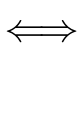
\includegraphics[scale=0.4,valign=t]{teste.png} }}%
    \qquad
    \begin{circuitikz} \draw
        (0,1) to[open,o-] (0,1) to (1,1) to[fullgeneric, l=$Z'$] (2,1) to (3,1) to[open,-o] (3,1)
        (0,0)
    ;
    \end{circuitikz}
    \caption{Estratégia para simplificação da malha.}
    \label{fig:ideia}
\end{figure}

\begin{equation}
    \label{eq2}
    \begin{cases}
        \overrightarrow{\nabla} \cdot \overrightarrow{J} \approx 0\\
        \overrightarrow{\nabla} \times \overrightarrow{E} = -\dfrac{\partial}{\partial t}\overrightarrow{B}
    \end{cases}
    \implies
    \begin{cases}
        \bar{I} = \bar{I}_{1} + \bar{I}_{2}\\
        \bar{U}_{1} = \bar{U}_{2} = \bar{U}_{malha}
    \end{cases}
\end{equation}

$$
    \begin{cases}
        \bar{I}_1 = \dfrac{1}{R_L + j\omega L}\ \bar{U}_1\\
        \bar{I}_2 = \dfrac{1}{1/(j\omega C_d)}\ \bar{U}_2
    \end{cases}
    \xRightarrow[]{\hyperref[eq2]{(2)}}
    \bar{I} = (\frac{1}{R_L + j\omega L} + \frac{1}{1/(j\omega C_d)})\bar{U}_{malha} 
$$

Aplicando a Lei de Ohm facilmente obtemos $\bar{Z}'$, i.e.:

$$
    \bar{Z}' = \frac{\bar{U}_{malha}}{\bar{I}} = \frac{(R_L + j\omega L)[1/(j\omega C_d)]}{R_L + j\omega L + [1/(j\omega C_d)]}
$$

De acordo com o plano, agora podemos analizar em conformidade com o conceito de circuito em série:

$$
\bar{U}_G = \bar{U}_R + \bar{U}_{malha} + \bar{U}_C \implies \bar{U}_G = (R_S + \frac{(R_L + j\omega L)[1/(j\omega C_d)]}{R_L + j\omega L + [1/(j\omega C_d)]} + \frac{1}{j\omega C})\ \bar{I}
$$

$$
\therefore \bar{Z}_{eq} = \frac{\bar{U}_G}{\bar{I}} = R_S + \frac{1}{j\omega C} + \frac{(R_L + j\omega L)[1/(j\omega C_d)]}{R_L + j\omega L + [1/(j\omega C_d)]}
$$
\hfill \ensuremath{\Box}

Supondo $R_L << \omega L$, temos que $R_L + j\omega L \approx j\omega L$, e assim obtemos a seguinte aproximação:

$$
\bar{Z}_{eq} = R_S + \frac{1}{j\omega C} + \frac{(j\omega L)[1/(j\omega C_d)]}{j\omega L + [1/(j\omega C_d)]} = R_S - j(\frac{1}{\omega C} + \frac{\omega L}{\omega^2 L C_d - 1})
$$

Para deduzir a nova frequência de ressonância, basta ter em consideração que o circuito durante o fenómeno é puramente resistivo, i.e., $\mathbb{I}m\{\bar{Z}_{eq}\} = 0$.

$$
\mathbb{I}m\{\bar{Z}_{eq}\} = 0
\implies
\frac{1}{\omega C} + \frac{\omega L}{\omega^2 L C_d - 1} = 0
\iff
\frac{1-\omega^2 L C_d}{\omega C(1-\omega^2 L C_d)} = \frac{\omega^2 L C}{\omega C(1-\omega^2 L C_d)}
$$

Para concluir, temos que a relação $1 = \omega^2 L C_d + \omega^2 L C$ deve ser satisfeita para certos $\omega$ (note-se que o denominador não se anula, evitando a singularidade).

$$
    \therefore \frac{1}{\omega^2} = L(C + C_d)
$$
\hfill \ensuremath{\Box}
%//==============================--@--==============================//%}
